\documentclass[aspectratio=149]{beamer}


\usepackage{lmodern}
\usepackage{amsmath}
\usepackage{hyperref}
\usepackage{booktabs}
\usepackage{url}
\usepackage{smartdiagram}
\usepackage{bm}
\usepackage{csquotes}
\usepackage{graphicx}
\usepackage[utf8]{inputenc}
\usepackage{amsmath}
\usepackage{lipsum}
\usepackage{float}
\usepackage{textgreek}
\usepackage{tikz}
\usepackage{datetime}
\usepackage[backend=bibtex,style=authoryear]{biblatex}
\usepackage{listings}
\usepackage{setspace}
\usepackage{braket}
\usepackage[font=small,format=plain,labelfont=bf,up,textfont=normal,up,format=hang]{caption}
\usecolortheme{crane}


\addbibresource{ref.bib}

\newdateformat{monthyeardate}{\footnotesize \monthname[\THEMONTH], \THEYEAR}
\title{Boundary Layer Receptivity to Freestream Disturbances}
\author[pawan]{\texorpdfstring{\\}{}
    Pawan Singh Negi \- \texorpdfstring{$174010003$}{}  \texorpdfstring{\\}{}
}
\institute[IITB]{Indian Institute of Technology, Bombay}


\begin{document}

\monthyeardate{}
\maketitle

%%%%%%%%%%%%%%%%%%%%%%%%%%%%%%%%%%%%

\begin{frame}
    \frametitle{Introduction}
    \begin{itemize}
        \item The receptivity of boundary layers concerns with the cause of
          instability rather it's evolution
        \item The boundary layers gets influenced by freestream turbulence,
          surface roughness, sound etc.
        \item no mathematical model that can predict the transition.
        \item boundary layers are convectively unstable i.e and unsteady
          distubance is required to generate the instability wave
    \end{itemize}
\end{frame}
%%%%%%%%%%%%%%%%%%%%%%%%%%%%%%%%%%%%
%%%%%%%%%%%%%%%%%%%%%%%%%%%%%%%%%%%%

\begin{frame}
    \frametitle{Path to Turbulence}
    \begin{figure}[h!]
      \centering
      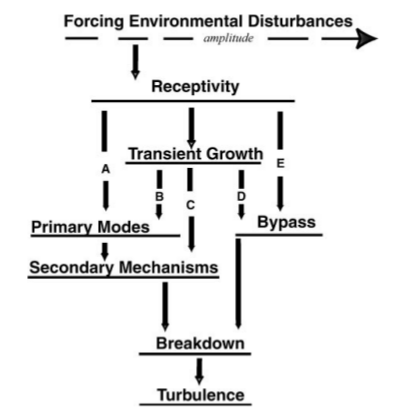
\includegraphics[scale=0.4]{path.png}
      \caption{Different possible paths to turbulence}
      \label{fig:path}
    \end{figure}
\end{frame}
%%%%%%%%%%%%%%%%%%%%%%%%%%%%%%%%%%%%   
%%%%%%%%%%%%%%%%%%%%%%%%%%%%%%%%%%%%

\begin{frame}
\frametitle{Tollmien-Schlichting (T-S) Waves}
    \begin{itemize}
        \item The Orr-Sommerfeld parallel flow inviscid approximation
  \begin{equation}
    (U-c)\left(\phi^{\prime \prime}-\alpha^{2} \phi\right)-U^{\prime \prime}
    \phi=-\frac{i}{\alpha \operatorname{Re}}\left(\phi^{\prime \prime \prime
    \prime}-2 \alpha^{2} \phi^{\prime \prime}+\alpha^{2} \phi\right),
    \label{eq:os}
  \end{equation}

        \item Rayleigh criterion That is $D^2U = 0$
        \item inviscid approximation are not suficient to predict
          instabilities in boundary layers.
    \end{itemize}
\end{frame}
%%%%%%%%%%%%%%%%%%%%%%%%%%%%%%%%%%%%
%%%%%%%%%%%%%%%%%%%%%%%%%%%%%%%%%%%%

\begin{frame}
\frametitle{Tollmien-Schlichting (T-S) Waves}
    \begin{itemize}
        \item using energy method that
  \begin{equation}
   \frac{D E}{D t}=-\int_{V} u^{\prime} v^{\prime}\left(\frac{d U}{d
   y}\right)-\frac{1}{R} \int_{V}\left(\nabla \vec{v}^{\prime}\right)^{2}.
    \label{eq:energy}
  \end{equation}
        \item in viscous flow $u^{'}$ and $v^{'}$ are non-orthogonal due
          to which viscosity becomes destabilizingdestabilizing
    \end{itemize}
\end{frame}
%%%%%%%%%%%%%%%%%%%%%%%%%%%%%%%%%%%%
%%%%%%%%%%%%%%%%%%%%%%%%%%%%%%%%%%%%

\begin{frame}
    \frametitle{Tollmien-Schlichting (T-S) Waves}
    \begin{figure}[h!]
      \centering
      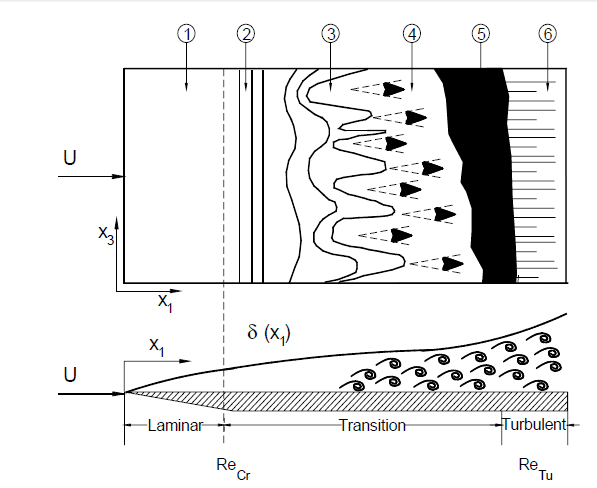
\includegraphics[scale=0.4]{xyz.png}
      \caption{T-S Wave on a flat plate}
      \label{fig:tswave}
    \end{figure}
\end{frame}
%%%%%%%%%%%%%%%%%%%%%%%%%%%%%%%%%%%%   
%%%%%%%%%%%%%%%%%%%%%%%%%%%%%%%%%%%%

\begin{frame}
    \frametitle{Receptivity Theory}
    \begin{itemize}
        \item An unsteady instability is required to generate instabilty in
          boundary layer.
        \item The unsteady instability can be naturally occuring or forced.
        \item Forced instability has broad wave spectrum, thus it can be
          used to appropriatly excite a particular mode.
        \item naturally occuring instabilities have concentrated
          wavenumbers, which is different then instability wave number thus
          they require a wavelength conversion process.
    \end{itemize}
\end{frame}
%%%%%%%%%%%%%%%%%%%%%%%%%%%%%%%%%%%%
%%%%%%%%%%%%%%%%%%%%%%%%%%%%%%%%%%%%

\begin{frame}
    \frametitle{Natural Receptivity}
    \begin{itemize}
        \item Leading edge region where the boundary layer is thin
        \item Downstream region, where some local feature causes the mean
          flow to adjust on a short streamwise length scale (e.g wall
          humps, suction strip).
    \end{itemize}
\end{frame}
%%%%%%%%%%%%%%%%%%%%%%%%%%%%%%%%%%%%
%%%%%%%%%%%%%%%%%%%%%%%%%%%%%%%%%%%%

\begin{frame}
    \frametitle{Leading Edge Receptivity}
    \begin{itemize}
        \item the Reynolds number is assumed to be large
        \item  The leading edge, where $x2 \pi f /U_\infty = O(1)$, the
          motion satisfies the linearized, unsteady, boundary-layer
          equation (LUBLE)
  \begin{equation}
   u_{t}^{\prime}+U u_{x}^{\prime}+V u_{y}^{\prime}+u^{\prime}
   U_{x}+v^{\prime} U_{y}=-p_{x}^{\prime}+\left(1 / R_{L}\right) u_{y
   y}^{\prime}.
    \label{eq:LUBLE}
  \end{equation}
        \item The LUBLE contains $u^{'} U_x$ and $V u^{'}_{y}$ which do not
          appear in the OSE.

    \end{itemize}
\end{frame}
%%%%%%%%%%%%%%%%%%%%%%%%%%%%%%%%%%%%
%%%%%%%%%%%%%%%%%%%%%%%%%%%%%%%%%%%%

\begin{frame}
    \frametitle{Leading Edge Receptivity}
    \begin{itemize}
        \item the first Lam-Rott asymptotic eigenfunction of the LUBLE,
          with coefficient $C_1$ , matches onto the T-S wave that becomes
          unstable farther downstream in the OSE region.
        \item  the finite nose radius weakens the influence of leading-edge
          scattering
        \item  An attractive feature of the leading- edge receptivity
          coefficient is that it is independent of frequency, f.

    \end{itemize}
\end{frame}
%%%%%%%%%%%%%%%%%%%%%%%%%%%%%%%%%%%%
%%%%%%%%%%%%%%%%%%%%%%%%%%%%%%%%%%%%

\begin{frame}
    \frametitle{Downstream Region Receptivity}
    \begin{itemize}
        \item Localized receptivity in the downstream is caused by the
          interaction of disturbances with short-scale variations in
          surface geometry.
        \item  the short-scale nonparallel mean-flow effects are again
          responsible for the transfer of energy from the wave- length of
          the freestream disturbance to that of the instability wave.
        \item  The OSE approach is only applicable for roughness elements
          of height $h/L << R^{-5/8}_{L}$, whereas the triple-deck analysis
          remains valid when $h/L = R^{-5/8}_{L}$.

    \end{itemize}
\end{frame}
%%%%%%%%%%%%%%%%%%%%%%%%%%%%%%%%%%%%
%%%%%%%%%%%%%%%%%%%%%%%%%%%%%%%%%%%%

\begin{frame}
    \frametitle{Computation Methods}
    \begin{itemize}
        \item the spatial direct numerical simula- tion (DNS) approach is
          widely applicable.
        \item  no restrictions with respect to the form or amplitude of the
          disturbances have to be imposed, because no linearizations or
          special assumptions concerning the disturbances have to be made.
        \item The complete integrated picture of geometry and associated
          pressure gradients (both favorable and adverse) must be included
          in any meaningful evaluation of receptivity, Thus DNS analysis is
          favourable.

    \end{itemize}
\end{frame}
%%%%%%%%%%%%%%%%%%%%%%%%%%%%%%%%%%%%
%%%%%%%%%%%%%%%%%%%%%%%%%%%%%%%%%%%%

\begin{frame}
    \frametitle{Experiments for Quatification}
    \begin{itemize}
        \item Large amplitude T-S wave
        \item Removable receptivity source
        \item Kendall gauge
        \item Complex plane resolution
        \item Resolution of duct acoustics
        \item Pulsed-sound technique

    \end{itemize}
\end{frame}
%%%%%%%%%%%%%%%%%%%%%%%%%%%%%%%%%%%%
\begin{frame}
    \centering
    Thank you
\end{frame}

\begin{frame}[t,allowframebreaks]
  \frametitle{References}
  \printbibliography{}
\end{frame}


%%%%%%%%%%%%%%%%%%%%%%%%%%%%%%%%%%%%

\end{document}
%%% Local Variables:
%%% mode: latex
%%% TeX-master: t
%%% End:
